\section{Web-app amministratori}
\subsection{Introduzione}
La web app costituisce l'interfaccia tramite la quale l'amministratore può interagire col sistema.
Le funzionalità offerte sono:
\begin{itemize}
	\item visualizzazione delle stanze e delle postazioni con i relativi stati;
	\item aggiunta, rimozione e modifica di stanze e postazioni;
	\item impostazione di postazioni come guaste;
	\item impostazione di stanze come inaccessibili;
	\item visualizzazione delle credenziali degli utenti;
	\item aggiunta, rimozione e modifica di credenziali;
	\item visualizzazione e scaricamento report sulle occupazioni e sulle igienizzazioni;
	\item visualizzazione di notifiche riguardanti il salvataggio dei dati sulla blockchain.
\end{itemize}

\subsection{Requisiti e installazione}

\subsection{Architettura}
L'architettura della web-app segue il modello a componenti imposto da Angular, che, a sua volta, si basa sul pattern Model-View-ViewModel, descritto dall'immagine sottstante.
\begin{figure}[H]
	\centering
	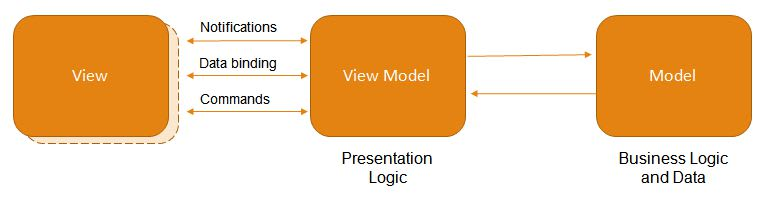
\includegraphics[width=15cm]{res/images/mvvm.jpg}
	\caption{Model-View-ViewModel}
	\label{fig:Model-View-ViewModel}
\end{figure}
Secondo questo modello la parte visiva del sito viene suddivisa in parti, e ognuna di queste parti viene controllata da una diversa classe.
La parte visiva viene chiamata view, mentre la parte di controllo viene chiamata view model.




